% Sune
%TODO:
% Apply defintiions
% Short introduction to Architecture qualities
As software engineers our focus is on creating a software architecture based on the architectural requirements. Software architecture allows us to reasons and take qualified decision. When designing BikeBus it is essential that we early in the project consider the architecture for the demands of the application. For this we will use known software principles to state measureable architectural demands. 

\subsection{Quality Attributes}
We will follow the definition on software architecture from \cite{Bass}. 
%**************************************Definition Software architecture
\begin{defi}[\textbf{Software architecture}]
The software architecture of a system is the set of \textbf{structures} needed to reason about the system, which comprise software \textbf{elements}, \textbf{relations} among them, and the \textbf{properties} of both. 
\end{defi}
%**************************************Definition Software architecture End


Our approach towards implementing a software architecture is based on Quality attribute (QA) and Quality attribute scenario (QAS). A quality attribute (QA) according to \cite{Bass} is as follows.

%**************************************Definition Quality attribute
\begin{defi}[\textbf{Quality attribute}]
..A quality attribute is a measurable or testable property of a system that is used to indicate how well the satisfies the needs of its stakeholders..  
\end{defi}
%**************************************Definition Quality attribute End


% TODO:
% Introduction to QA
% List relevant quality attributes
% Why these attributes?
% Relate to generel mobile application challenges and tactics

From \cite{Bass} we have seven quality attributes here among modifiability, availability and performance. Furthermore \cite{Kjaergaard:2015:AQT:2737182.2737196} has added energy efficiency and ressources adaptability.  


We will discuss different tactics on software architecture for achieving the requirements for the BikeBus application. A tactic according to \cite{Bass} is defined as.

%**************************************Definition Tactic
\begin{defi}[\textbf{Tactic}]
Tactic is a design decision that influences the achievement of a quality attribute response. 
\label{def:tactic}
\end{defi}
%**************************************Definition Tactic End

\subsubsection{Quality Attribute Scenarios}
% TODO:
% Formal definition of QAS
% Use template from Bass

A core observation is that a QA should be measurable or testable quality. The key point is when working with QA we use them in a given context/scenario and therefor we informally call these as QAS.\\



\begin{figure}[H]
\centering
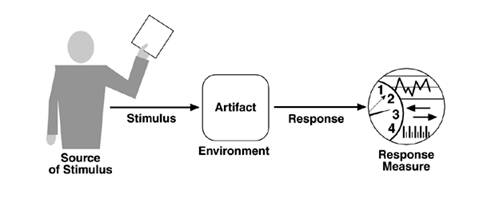
\includegraphics[scale=0.5]{QualityAttributeScenario.jpg}

\caption{The parts of a quality attribute scenario}
\label{fig:Quality_Attribute_Scenario}
\end{figure}






One of the core aspects of the definition of software architecture, is that software architecture is a set of structures, which we can use to reason about the system. To assist and visualize these structures, elements, relations and properties we use relevant viewpoints. These viewpoint originates from $3+1$ article \cite{3+1}, where the $+1$ is the architectural requirements. These architectural requirements can be formulated through QAS.


In the following we formulated a modifiability, a energy efficiency and a ressource adaptablity QAS for the BikeBus application. We chose to focus on modifiability because we want Bikebus to be easily modifiable when new changes has to be made. We chose to focus on energy efficiency because we have limited battery available on the phone and resource adaptability because the BikeBus is depended on network resources.

According to \cite{Bass} modifiability is defined as follows from definition \ref{def:modifiability}. It means more formel that we need to somehow quantify how well BikeBus adapts to changes.

%**************************************Definition modifiability
\begin{defi}[\textbf{Modifiability}]
..Concerned with the ease with which the system supports change..  
  \label{def:modifiability}
\end{defi}
%**************************************Definition modifiability End

 For now BikeBus relies on Google API framework for retrieving locations. To be able to adapt, with all the different sensor frameworks available, an QAS (table \ref{table:modifiability_qas}) is formulated for this demand. 

\begin{table}[H]
\begin{center}
\begin{tabular}{|p{0.3cm}|p{2.5cm}|p{8cm}|}
  \hline
  \multicolumn{2}{|p{3cm}|}{\bfseries Scenario(s):} & \#  1: A developer should be able to replace sensor frameworks during runtime and apply the changes within 30 minutes. \\
  \hline
  \multicolumn{2}{|p{3cm}|}{\bfseries Relevant Quality Attributes:} & Modifiability\\
  \hline
  \multirow{6}{*}{\begin{sideways}{\bfseries Scenario Parts}\end{sideways}}
  & {\bfseries Source:} & Developer \\
  \cline{2-3}
  & {\bfseries Stimulus:} & Needs to replace a sensor frameworks \\
  \cline{2-3}
  & {\bfseries Artifact} &  Code \\
  \cline{2-3}
  & {\bfseries Environment:} &  Design time \\
  \cline{2-3}
  & {\bfseries Response:} &  Replacement made\\
  \cline{2-3}
  & {\bfseries Response Measure:} & In 30 minutes\\
  \hline
\end{tabular}
\caption{Modifiability QAS}
\label{table:modifiability_qas}
\end{center}
  
\end{table}

\cite{Kjaergaard:2015:AQT:2737182.2737196} defines energy efficiency as follows from figure \ref{def:energy_efficiency}. Energy efficiency is vital to take into consideration when developing mobile application since there are rarely turned off.  

%**************************************Definition Energy efficiency
\begin{defi}[\textbf{Energy efficiency}]
Energy efficiency the "amount" of energy required to provide and/or deliver a (mobile)
service at a given quality of service (QoS).  
  \label{def:energy_efficiency}
\end{defi}
%**************************************Definition Energy efficiency End

From the literature \cite{Kjaergaard2010} it is known that sensors such as GPS is an energy consumer. Since BikeBus is tightly connected to locations through the GPS, the application needs to be energy efficient such that the application doesent drains a fully loaded battery. The QAS in table \ref{table:energi_efficiency_qas} is about energy consumption per event. We are aware of other scenarios which a production application also needs to take into account such as low battery.

\begin{table}[H]
\begin{center}
\begin{tabular}{|p{0.3cm}|p{2.5cm}|p{8cm}|}
  \hline
  \multicolumn{2}{|p{3cm}|}{\bfseries Scenario(s):} & \#  2: Using the app for twenty minutes should result in a discharge rate of 6 \% average per hour.  \\
  \hline
  \multicolumn{2}{|p{3cm}|}{\bfseries Relevant Quality Attributes:} & Energy efficiency\\
  \hline
  \multirow{6}{*}{\begin{sideways}{\bfseries Scenario Parts}\end{sideways}}
  & {\bfseries Source:} & Events \\
  \cline{2-3}
  & {\bfseries Stimulus:} & Arrives periodically \\
  \cline{2-3}
  & {\bfseries Artifact} &  BikeBus application \\
  \cline{2-3}
  & {\bfseries Environment:} &  High energy availability \\
  \cline{2-3}
  & {\bfseries Response:} &  Process data\\
  \cline{2-3}
  & {\bfseries Response Measure:} & Discharge rate of 6 \% average per hour \\
  \hline
\end{tabular}
\caption{Energi efficiency QAS}
\label{table:energi_efficiency_qas}
\end{center}
\end{table}

According to \cite{Kjaergaard:2015:AQT:2737182.2737196} resource adaptability is defined as follows from definition \ref{def:resource_adaptability}. It means more formal that we need to somehow quantify how well BikeBus adapts to changes in the environment. Often the phone is in motion, so we cant be sure of having good network coverage all the time. Since BikeBus is depended on GPS signal over the network when biking, the application needs to be able to handle no network coverage. In other words BikeBus needs to react on this change which effects the quality of service.    

%**************************************Definition Energy efficiency
\begin{defi}[\textbf{Resource adaptability}]
Resource adaptability is the ability of services to flexibly adapt to changing environments given by fluctuating availability of sensing and communication resources with different QoS levels, context-dependent quality of sensing data, and fluctuating wireless communication options and network availability/accessibility.  
  \label{def:resource_adaptability}
\end{defi}
%**************************************Definition Energy efficiency End

The way BikeBus handles the change in environment is by switching from opportunistic to participatory sensing, which is formulated in table  \ref{table:resource_adaptability_qas}. The idea is if the location services isnt available, then the user himself must turn on when the route starts and ends. This isnt an optimal solution but it is reasonable solution. The accuracy will not be the same and the data collection will also lack, but the application will still be able to calculate basic statistics.    

\begin{table}[H]
\begin{center}
\begin{tabular}{|p{0.3cm}|p{2.5cm}|p{8cm}|}
  \hline
  \multicolumn{2}{|p{3cm}|}{\bfseries Scenario(s):} & \#  3: When the network coverage disappears from the phone, the BikeBus application has fewer resources available and changes the level of service by initiating participatory sensing and degrading the average accuracy level to 80\%. \\
  \hline
  \multicolumn{2}{|p{3cm}|}{\bfseries Relevant Quality Attributes:} & Resource adaptability\\
  \hline
  \multirow{6}{*}{\begin{sideways}{\bfseries Scenario Parts}\end{sideways}}
  & {\bfseries Source:} & Changes in network signal \\
  \cline{2-3}
  & {\bfseries Stimulus:} & No network coverage  \\
  \cline{2-3}
  & {\bfseries Artifact} &  BikeBus \\
  \cline{2-3}
  & {\bfseries Environment:} &  Few resources \\
  \cline{2-3}
  & {\bfseries Response:} &  Change level of service to participatory sensing\\
  \cline{2-3}
  & {\bfseries Response Measure:} & Degraded service level with an accuracy on average of 80\%\\
  \hline
\end{tabular}
\caption{Resource Adaptability QAS}
\label{table:resource_adaptability_qas}
\end{center}
\end{table}


\subsection{Tactics}
% TODO:
% For each QA find tactics
% Examples
%   - Performance: Limit sampling rate
%       - Possible solution: Our hierarachy divide and 
%         conquer
%   - Modifiability: Encapsulation/coupling/cohesion
%       - Possible solution: Interfaces, multiple APIs 
%         and storage
%   - Availability: Redundancy (caching layer)
%       - Possible solution: local caching
This section is about tactics which satisfies the response measure in the QAS. As stated in definition \ref{def:tactic} - a tactic is a design decision that influences the achievement of a quality attribute response. For each tactic there will be a description and an argument of the choosen tactic. 

\subsubsection{Modifiability}
\label{subsec:modifiability}
 Modifiability is concerned with the ease with which the system supports change. By programming to an interface around the sensor implementations, we have used the tactic \textit{Encapsulate} \cite{Bass} and efficiently encapsulated this functionality and made the system ready to change to other sensor frameworks. There are implementations of activity regocnition, location and geofence which needs to be encapsulated behind interfaces. The process which identify the need for implementing interfaces is as follows \cite{Baerbak10}: 

\begin{enumerate}
    \item Identify the behavior that varies. 

    \item Use interface which encapsulate the variable behavior.     
    
    \item Delegate the responsibility to a specialized classes.
\end{enumerate}
 
 
 
\subsubsection{Energy Efficiency}
\label{subsec:energy_efficiency}
To fulfill the energy efficiency QAS the sensor replacement tactic \cite{Kjaergaard:2015:AQT:2737182.2737196} is chosen to improve the energy consumption of the application .The idea is that a least costly sensor triggers another more energy consuming sensor. To achieve sensor replacement the activity recognition is first triggered and if it returns biking the location api is activated. From the literature \cite{Kjaergaard2010} it is a known fact that activating the GPS/radio consumes a certain amount of power. This implementation is arguable in different contexts. Sensor replacement could potentially cause unnecessary energy consumption. Since it is a biking application why bother for recognizing the biking activity. By doing activity recognition also gives better accuracy, since biking also involves holding for red lights etc. 

BikeBus is tested, which resulted in an average discharge rate on 5.44 \%. The battery was fully loaded and it was monitored by battery historian. With a discharge rate off 5.44\% it holds the response measure stated in QAS table \ref{table:energi_efficiency_qas}. 

%The app is tested with 6 biking trips which resulted in an average discharge rate on 5.44 %. The battery was monotoring by battery historian. 


% keywords:
% - Use one sensor to decide if the location sensor should be used
% - Discussion about which sensor should decide if the location sensor should be used
%    - Activity Recognition: Might be more expensive than location itself but has high accuracy
%    - Significant motion sensor: Very low energy consumption, but does not check for biking (assume we are biking when collecting on a bikebus)
% - If there was a qas for accuracy this could be prototyped and tested, but if both activity rec and significant comply with the qas then there is no problem

%Evt: performance test with battery historian

\subsubsection{Resource Adaptability}
If their are poor network coverage, then the user will be prompted to manually "start" the beginning and "end" the route. In this way BikeBus will still be functional and the user will be able to use the application. Since BikeBus under normal condition uses activity recognition together with location it will switch to use the accelerometer, if network coverage is poor. The accelerometer will then supply data about the motion of the user. BikeBus will then in some sense be able to sort out data when the user isnt in motion. Resource selection  \cite{Kjaergaard:2015:AQT:2737182.2737196} will be applied, choosing between activity recognition together with location to the accelerometer. This isnt an optimal solution. Other more drastic solution could be that network coverage is a requirement. The Google I/O is an example that requires NFS which was a solution due to phones hardware constrains \cite{Barnett2015}.     

This feature is not implemented yet. This is an idea for feature work.


